\documentclass{article}
\usepackage[a4paper, bindingoffset=0 cm, left=2.5cm, right=2.5cm, top=1.5cm, bottom=1.5cm, footskip=0.5cm]{geometry}
\usepackage[utf8]{inputenc}
\usepackage[english]{babel}
\usepackage{mdframed}
\usepackage{tikz}
\usepackage{biblatex}
\usepackage{csquotes}
\addbibresource{literature.bib}
\usepackage{hyperref}
% Added for the figures and tables of this paper
\usetikzlibrary{positioning,arrows.meta}
\usepackage{graphicx}
\usepackage{booktabs}
\usepackage{amsmath}
\usepackage{caption}
\usepackage{subcaption}

\title{1JM0211 Process Mining \\Mining Organizational Patterns}
\author{Group 5, Members: Sophie Veltmans, Lotte van der Vlies, Gijs Kruize}
\date{Submission Date}

\begin{document}
\newmdenv[linewidth=1.5pt, frametitlerule=true, roundcorner=3pt]{mybox}
\pagestyle{empty}
\let\svmaketitle\maketitle
\def\maketitle{\svmaketitle\thispagestyle{empty}}
\maketitle

\begin{mybox}[frametitle = Remarks (to be removed upon submission)]
Page limit: 5 pages excluding references; use appropriate scientific references where possible \cite{DBLP:books/sp/Aalst16}; your short paper shall follow the structure outlined below
\end{mybox}

% =====================================================================
\section{Motivation and Scientific Background}\label{sec:motivation}

Process mining discovers, checks and improves processes from the events that
information systems record~\cite{DBLP:books/sp/Aalst16}. Most of its
techniques focus on the control flow: which activities happen in which order.
\emph{Organizational mining} adds the actors: it asks who performs which
activities, which resources play similar roles and how work is handed over
between them~\cite{song2008organizational}. Classical results are role and
team discovery and social networks such as the handover-of-work
network~\cite{vanderaalst2005social}. These describe relations between actors,
but not \emph{which tasks} the actors perform together and in which structure.

A direct way to combine both perspectives is to label each event with an
activity--resource pair and to discover a process model on these labels. With
many resources this produces large, unreadable ``spaghetti'' models.
Diamantini et al.~\cite{diamantini2016behavioral} therefore propose
\emph{behavioral process mining}: build one \emph{instance graph} per case,
which shows the order and the parallelism of its events, and mine the most
relevant subgraphs over all instance graphs. Such a subgraph, a
\emph{behavioral pattern}, is a recurring work practice: for example, ``two
clerks complete the application in parallel, after which a manager decides''.

\paragraph{Running example.} In the loan application process of the BPI
Challenge 2017~\cite{vandongen2017bpi}, an application is submitted online,
completed by phone, an offer is sent, and the returned offer is validated
before a decision is made. A pattern such as ``the offer team calls the
customer, after which the validation team takes over'' tells an analyst how
the work is divided, which a model on activities alone cannot show.

\paragraph{Relation to the course.} The approach combines several course
topics: event log preprocessing and event abstraction (choosing the label),
process discovery (the Inductive Miner~\cite{leemans2014infrequent}),
conformance checking (BIG aligns every trace with the model to repair irregular
instance graphs~\cite{diamantini2016big,adriansyah2011alignments}) and
organizational mining (roles and handovers). Unlike process discovery, it does
not aim at one model for all cases; unlike social network analysis, it keeps
the tasks and their order in the result.

\paragraph{Contribution.} We (i) implement the complete pipeline of
Figure~\ref{fig:pipeline} with pm4py~\cite{berti2019pm4py}, BIG and SUBDUE,
(ii) group resources into discovered roles to keep the approach tractable and
interpretable, (iii) speed up SUBDUE without changing its results, and (iv)
evaluate the patterns against a gold standard and a baseline.

% =====================================================================
\section{Conceptual Approach}\label{sec:conceptual_approach}

\begin{figure}[t]
\centering
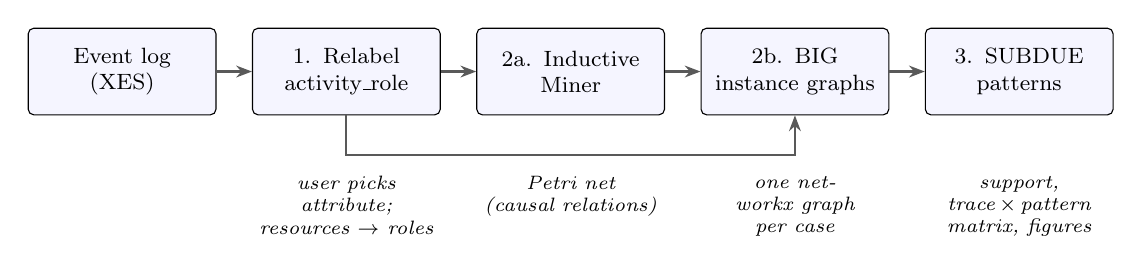
\begin{tikzpicture}[
  box/.style={draw, rounded corners=2pt, align=center, font=\footnotesize,
              minimum height=1.1cm, text width=2.15cm, fill=blue!4},
  data/.style={font=\scriptsize\itshape, align=center, text width=2.3cm},
  arr/.style={-{Stealth[length=2mm]}, thick, gray!70!black}]
\node[box] (log) {Event log\\(XES)};
\node[box, right=0.45cm of log] (pre) {1. Relabel\\activity\_role};
\node[box, right=0.45cm of pre] (net) {2a. Inductive\\Miner};
\node[box, right=0.45cm of net] (big) {2b. BIG\\instance graphs};
\node[box, right=0.45cm of big] (sub) {3. SUBDUE\\patterns};
\draw[arr] (log) -- (pre);
\draw[arr] (pre) -- (net);
\draw[arr] (net) -- (big);
\draw[arr] (big) -- (sub);
\draw[arr] (pre.south) |- ++(0,-0.5) -| (big.south);
\node[data, below=0.65cm of pre] {user picks attribute;\\resources $\to$ roles};
\node[data, below=0.65cm of net] {Petri net\\(causal relations)};
\node[data, below=0.65cm of big] {one networkx graph\\per case};
\node[data, below=0.65cm of sub] {support, trace\,$\times$\,pattern\\matrix, figures};
\end{tikzpicture}
\caption{Pipeline. Step~1 relabels every event with its activity and the role of
the selected attribute; step~2 discovers a Petri net and builds one instance
graph per case with BIG; step~3 mines behavioral patterns with SUBDUE.}
\label{fig:pipeline}
\end{figure}

\subsection{Step 1: event log preprocessing}

\paragraph{Input.} An event log in XES format; each event has at least a case
identifier, an activity (\texttt{concept:name}) and a timestamp, plus further
attributes. Trace attributes are copied to every event of the case.

\paragraph{Attribute selection and relabelling.} The tool lists all attributes
of the log with their level (event or trace), number of distinct values, share
of events that have a value and examples, and asks the user on the command
line which attribute to analyse. Every event is then relabelled as
\texttt{activity\_value}, e.g.\ \texttt{A-Submitted\_User\_1}: an instance of an
\emph{entity specification} (activity, executor) in the terms
of~\cite{diamantini2016behavioral}. Missing values become \texttt{UNKNOWN} so no
event is lost, and whitespace is replaced because BIG's output format is space
separated. The original activity and value are kept as separate attributes,
because a label such as \texttt{A-Submitted\_User\_1} cannot be split back
unambiguously.

\paragraph{Grouping resources into roles.} With \texttt{org:resource} the BPI
log has 134 users and 3,338 distinct labels; almost half of these labels occur
fewer than 10 times. Such fine labels make discovery and BIG slow and spread
the same behaviour over many labels, so few patterns are frequent. Optionally,
the values are therefore replaced by \emph{roles} discovered with the method of
Burattin et al.~\cite{burattin2013roles} (pm4py): every activity starts as a
role, described by the multiset of resources that perform it, and the two roles
with the most similar (normalised) resource multisets are merged as long as
their similarity exceeds a threshold $\theta$ (default $0.65$). A resource can
belong to several of the resulting roles; we assign it its \emph{dominant
role}, the one in which it performs most of its events. Labelling an event with
the role of its \emph{activity} instead would add no information beyond the
activity itself; the dominant role of the \emph{resource} also shows when
somebody works outside their usual role.

\paragraph{Output.} The relabelled log (XES) plus tables of the roles, the
role of every resource and the frequency of every label.

\subsection{Step 2: instance graphs}

An instance graph~\cite{vandongen2004instance} represents one case as a
directed acyclic graph: nodes are the events, edges the causal order between
them. Events that may happen in any order are placed on parallel branches
instead of in their arbitrary recorded order. The causal relations come from a
process model, which we discover with the \emph{infrequent} Inductive
Miner~\cite{leemans2014infrequent} on the relabelled log (noise threshold
$0.2$, ProM's default, as in~\cite{diamantini2016behavioral}). The provided BIG
library~\cite{diamantini2016big} aligns every trace with this Petri net, builds
its instance graph and repairs the graphs of traces that do not fit the model
(inserted and deleted events). BIG writes all graphs to one text file
(\texttt{.g}), one block per case with local node ids.

We convert this file to one \texttt{networkx} graph per case. Every node gets a
\emph{unique global id}; the local id is kept as an attribute and all edges are
translated through the same mapping, so all relations are preserved. Because
the \texttt{.g} file does not name the cases, graph $i$ is linked to case $i$ of
the log. Every node carries its label, activity and role.

\subsection{Step 3: behavioral patterns with SUBDUE}

All instance graphs are given to SUBDUE~\cite{cook1994subdue,jonyer2002subdue}
as one disconnected graph. Nodes are matched on their label; all edges get the
same label and are directed. SUBDUE searches, with a beam search, the subgraph
that best compresses this graph. The Python implementation we use scores a
pattern $s$ with $k$ non-overlapping instances and $|E_s|$ edges in a graph
with $|E|$ edges as
\begin{equation}
  \text{value}(s) = \frac{(k-1)\,|E_s|}{|E|},
\end{equation}
so frequent and large patterns score highest, in the spirit of the minimum
description length criterion of~\cite{diamantini2016behavioral}. With more than
one \emph{iteration}, every instance of the best pattern is compressed into a
single node and the search is repeated; later patterns can contain earlier ones,
which yields the pattern hierarchy of~\cite{diamantini2016behavioral}.

\paragraph{Parameters.} Beam width (number of candidates kept per level, 4 as
in~\cite{diamantini2016behavioral}), minimum and maximum pattern size (2 and 10
edges), number of reported patterns per iteration, number of iterations, and
\emph{limit}, the number of candidates SUBDUE extends. The Python SUBDUE starts
from all one-edge patterns in the order of the edges, not by value, and stops
after \emph{limit} extensions; a small limit thus makes the result depend on
the arbitrary edge order. We therefore set it automatically to the number of
one-edge patterns plus beam width times maximum size, so that every one-edge
pattern is extended once and the beam can reach the maximum size.

\paragraph{Output.} For every pattern: its graph, the number of instances
(occurrence-based support, as in~\cite{diamantini2016behavioral}), the number
and share of cases that contain it (transaction-based support), its roles, and
a \emph{trace $\times$ pattern matrix} with a 1 when the pattern occurs in the
case. Visualisation functions draw instance graphs and patterns (roles by
colour and tag), the support per pattern, the overlap between patterns and the
handover of work between roles.

% =====================================================================
\section{Implementation}\label{sec:implementation}

The pipeline is a Python~3.9 package with one module per step and a single
command-line entry point (\texttt{main.py}); all parameters are command-line
options and the README lists the exact commands. pm4py~2.2.16 is used as BIG
requires. Three implementation details matter for the results:

\begin{itemize}
\item \textbf{Reproducibility.} pm4py's Inductive Miner iterates over Python
sets, whose order changes between runs, so the discovered Petri net could
differ between two runs on the same log. The program fixes the hash seed, after
which repeated runs give identical instance graphs.
\item \textbf{BIG in parallel.} BIG processed about 15 cases per minute (3.5
hours for the log). Because it treats every case independently, we run the
unmodified BIG on consecutive chunks of the log in parallel processes and
concatenate the outputs in order; the result is byte-for-byte identical to a
single run, in 49 minutes on 11 cores.
\item \textbf{SUBDUE speed-up.} SUBDUE compares candidates pairwise (every edge
with every edge, every extended instance with every other), which is quadratic.
Without changing SUBDUE's code we replace three helper functions at run time:
candidates are first grouped by a fingerprint that every pair of matching
graphs shares (vertex labels with degree, edge labels), SUBDUE's own graph
matcher decides within a group, and overlap is tested against a set of used
vertices. Groups are processed in the original order, so the output (patterns,
values and instances) is identical; this is verified by unit tests and on the
data (Table~\ref{tab:performance}). We also found that SUBDUE's networkx
interface silently makes all edges undirected, so we build its input directly.
\end{itemize}

\begin{table}[t]
\centering
\caption{SUBDUE run time on the first $N$ instance graphs (beam 4, max.\ size 10).
Both versions return identical patterns and instances.}
\label{tab:performance}
\begin{tabular}{rrrrr}
\toprule
Instance graphs & Edges & Original & Accelerated & Speed-up \\
\midrule
250 & 9,898 & 23.6\,s & 11.0\,s & 2.1$\times$ \\
1,000 & 39,221 & 282.4\,s & 63.2\,s & 4.5$\times$ \\
3,093 (all) & 121,781 & not run & 142.7\,s & -- \\
\bottomrule
\end{tabular}
\end{table}

% =====================================================================
\section{Evaluation Design and Results}\label{sec:evaluation}

\subsection{Data}

We use the provided subset of the BPI Challenge 2017
log~\cite{vandongen2017bpi}: 3,093 loan applications that were denied, with
124,866 events, 54 activities and 19 attributes. Activity names start with
\texttt{A-} (application states), \texttt{O-} (offer states) or \texttt{W-}
(work items, whose lifecycle step is part of the name, e.g.\
\texttt{W-Validate-application-start}). We analyse the attribute
\texttt{org:resource} (134 users, one of which, \texttt{User\_1}, is the
system). Other attributes are less suited: \texttt{EventOrigin} is determined
by the activity and adds no information, and trace attributes such as the loan
goal are constant within a case, so they split the cases into groups but cannot
show any handover.

\subsection{Evaluation design}

\paragraph{Gold standard.} We built a gold standard of 9 expected work
practices (Table~\ref{tab:gold}) from the process phases in the log
description (submission, completion by phone, offer, assessment of the returned
offer, incomplete files, decision), the lifecycle order of the BPI~2017
activities, and the role that performs most of each activity according to the
\emph{step~1} role table (Figure~\ref{fig:roles}). Two of them are handovers
between roles. The gold standard is thus derived independently of the SUBDUE
output; however, it was written after we had seen preliminary results, which we
discuss as a limitation.

\begin{table}[t]
\centering
\caption{Gold standard: expected work practices (R$k$ = Role\_$k$).}
\label{tab:gold}
\small
\begin{tabular}{lll}
\toprule
ID & Work practice & Roles \\
\midrule
G1 & Application submission: start $\to$ create $\to$ submitted & R4 \\
G2 & Lead handling after submission & R4 \\
G3 & Concept created, completion started by phone (\emph{handover}) & R4 $\to$ R1 \\
G4 & Application accepted, offer created and sent & R1 \\
G5 & Calling the customer after the offer & R1 \\
G6 & Call aborted when the offer returns (\emph{handover}) & R1 $\to$ R2 \\
G7 & Validation scheduled, started, validating & R2 \\
G8 & Calling the customer for incomplete files & R3 \\
G9 & Final decision: denied, offer refused & R3 \\
\bottomrule
\end{tabular}
\end{table}

\paragraph{Measures.} A gold pattern is \emph{found} if a discovered pattern
contains it as a labelled subgraph; a discovered pattern is \emph{correct} if it
contains a gold pattern or is part of one. Precision is the share of correct
discovered patterns, recall the share of found gold patterns; we also report
F1 and, as partial credit, precision and recall on edge level (pairs of
labels). Following~\cite{diamantini2016behavioral} we further report the
support of the patterns.

\paragraph{Configurations and baseline.} We compare a single SUBDUE iteration
(20 best patterns) with a hierarchical run of 10 iterations (3 patterns each),
and vary the beam width (4, 10, 20) as in~\cite{diamantini2016behavioral}. As a
simple baseline we take the most frequent label paths of 2, 3 and 4 edges in the
instance graphs (as many as SUBDUE returns), which corresponds to sequential
pattern mining without compression.

\subsection{Results}

\paragraph{Roles.} Role discovery groups the 134 users into 8 roles
($\theta=0.65$), reducing the labels from 3,338 to 225. The four large roles are
interpretable (Figure~\ref{fig:roles}): Role\_1 (86 users) completes
applications and creates, sends and follows up offers; Role\_2 (21 users)
validates returned offers; Role\_3 (18 users) handles fraud checks, incomplete
files and denials; Role\_4 (2 users, including the system user) registers
applications. 32 of the 54 activities are performed for more than 90\% by a
single role.
Roles 5--8 are small (3, 2, 1 and 1 users, the last two with 6 and 1 events)
and are artefacts of the dominant-role assignment.

\begin{figure}[t]
\centering
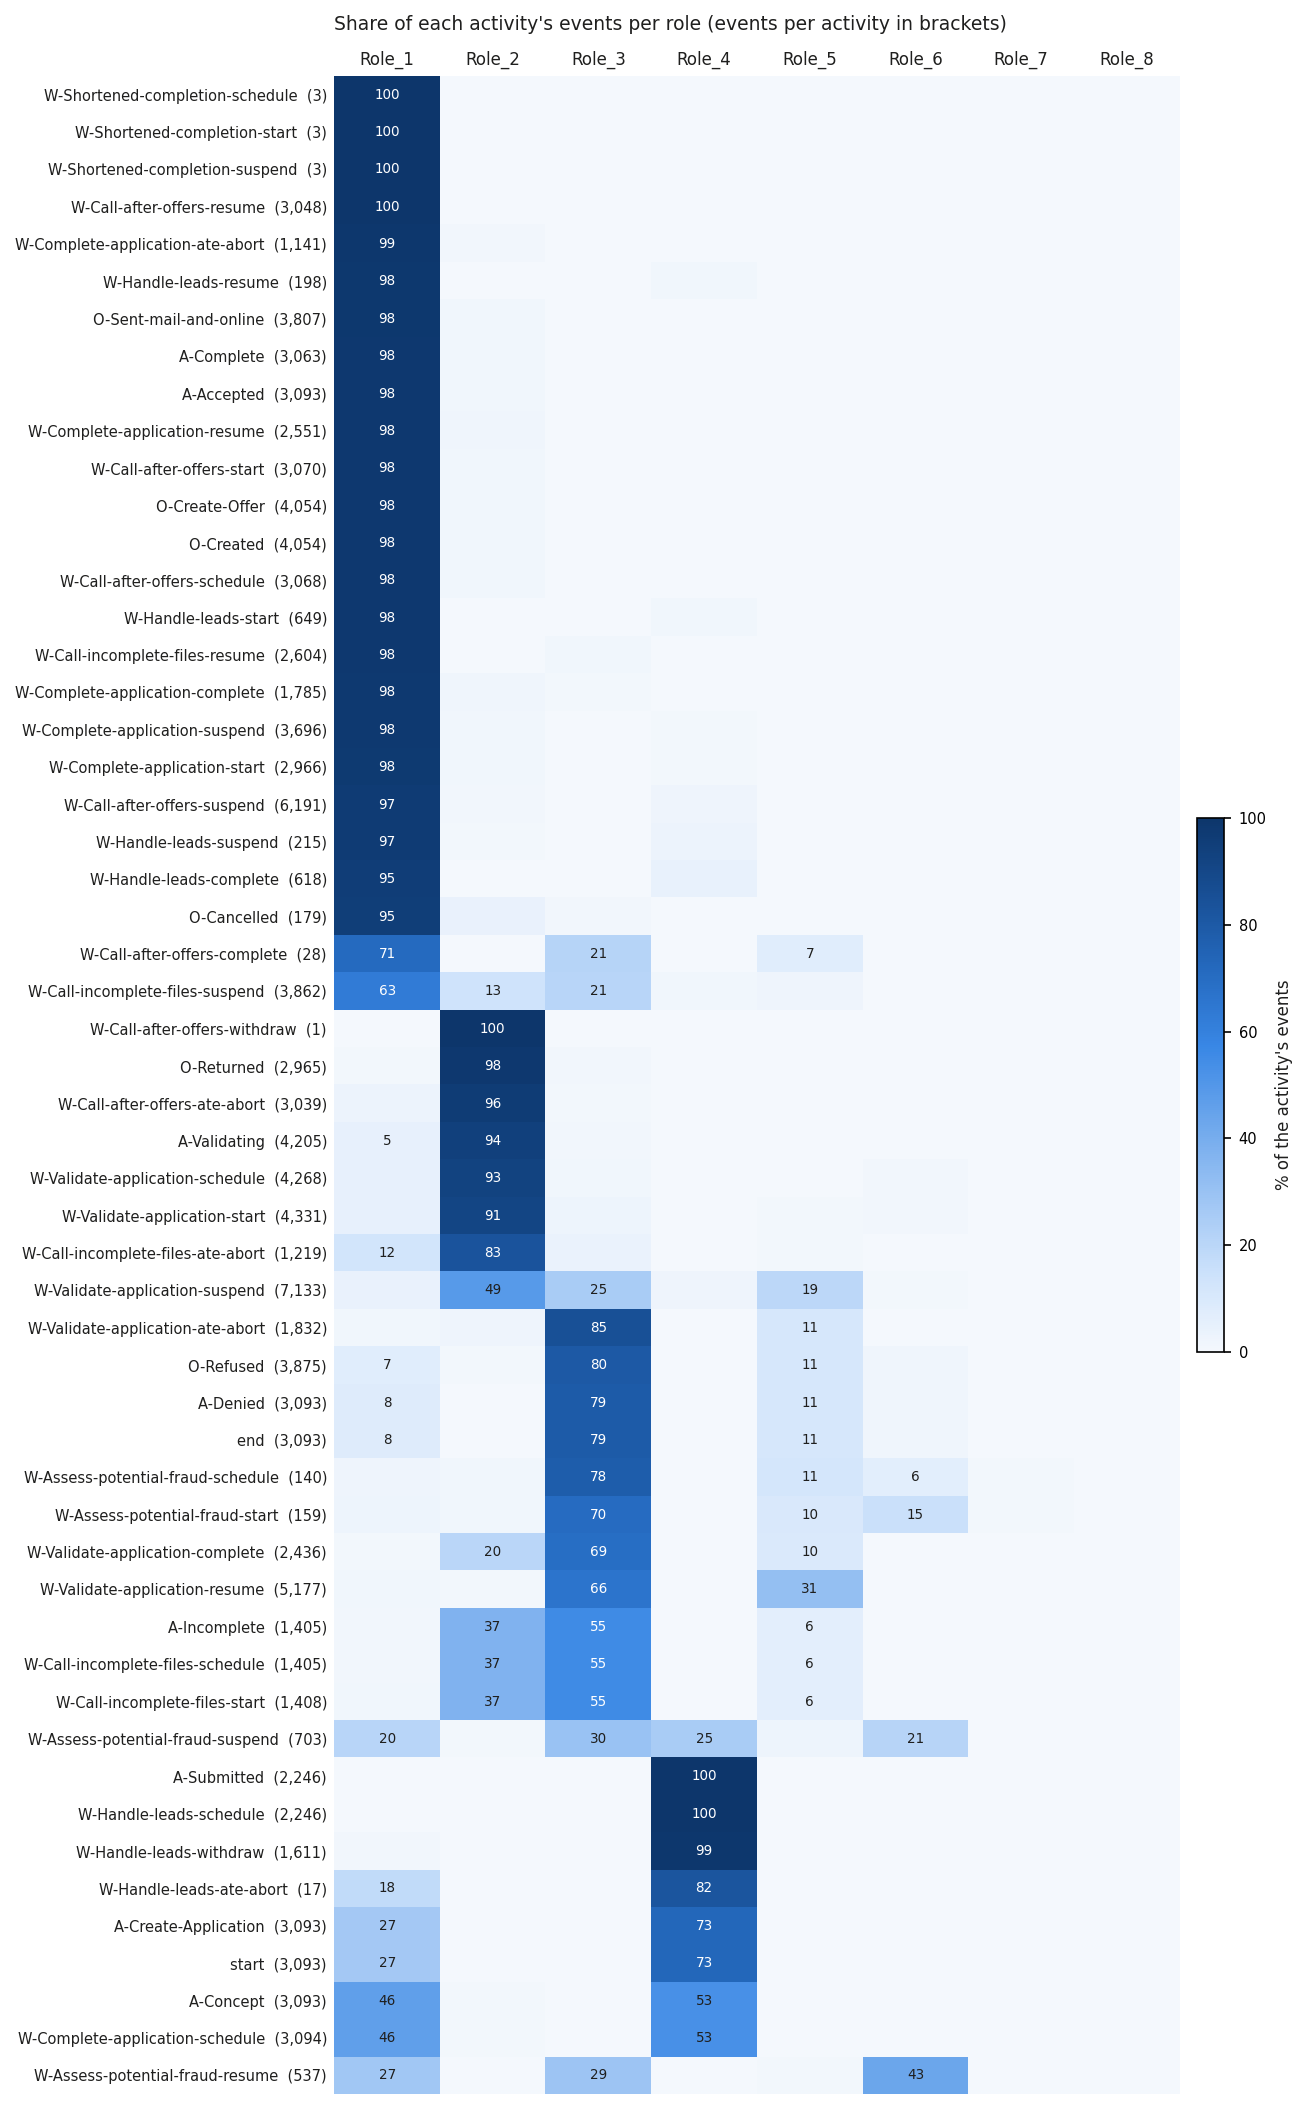
\includegraphics[width=0.62\textwidth]{figures/roles_per_activity.png}
\caption{Share of each activity's events performed by each discovered role
(step~1). Each block of dark cells is the work of one role.}
\label{fig:roles}
\end{figure}

\paragraph{Instance graphs.} BIG produced 3,093 instance graphs (one per case)
with 124,866 nodes and 121,781 edges, all connected. Only 0.3\% contain parallel
branches: the discovered Petri net (219 visible and 134 silent transitions) has
a single AND-split. This is \emph{not} caused by the roles: the same miner on
the plain activities, at any noise threshold between 0 and 1, also finds one
AND-split, whereas the Petri net provided with the assignment has five and its
instance graphs are parallel in 99.3\% of the cases. Figure~\ref{fig:ig} shows a
typical instance graph, in which the case passes from Role\_4 to Role\_1,
Role\_2 and Role\_3.

\begin{figure}[t]
\centering
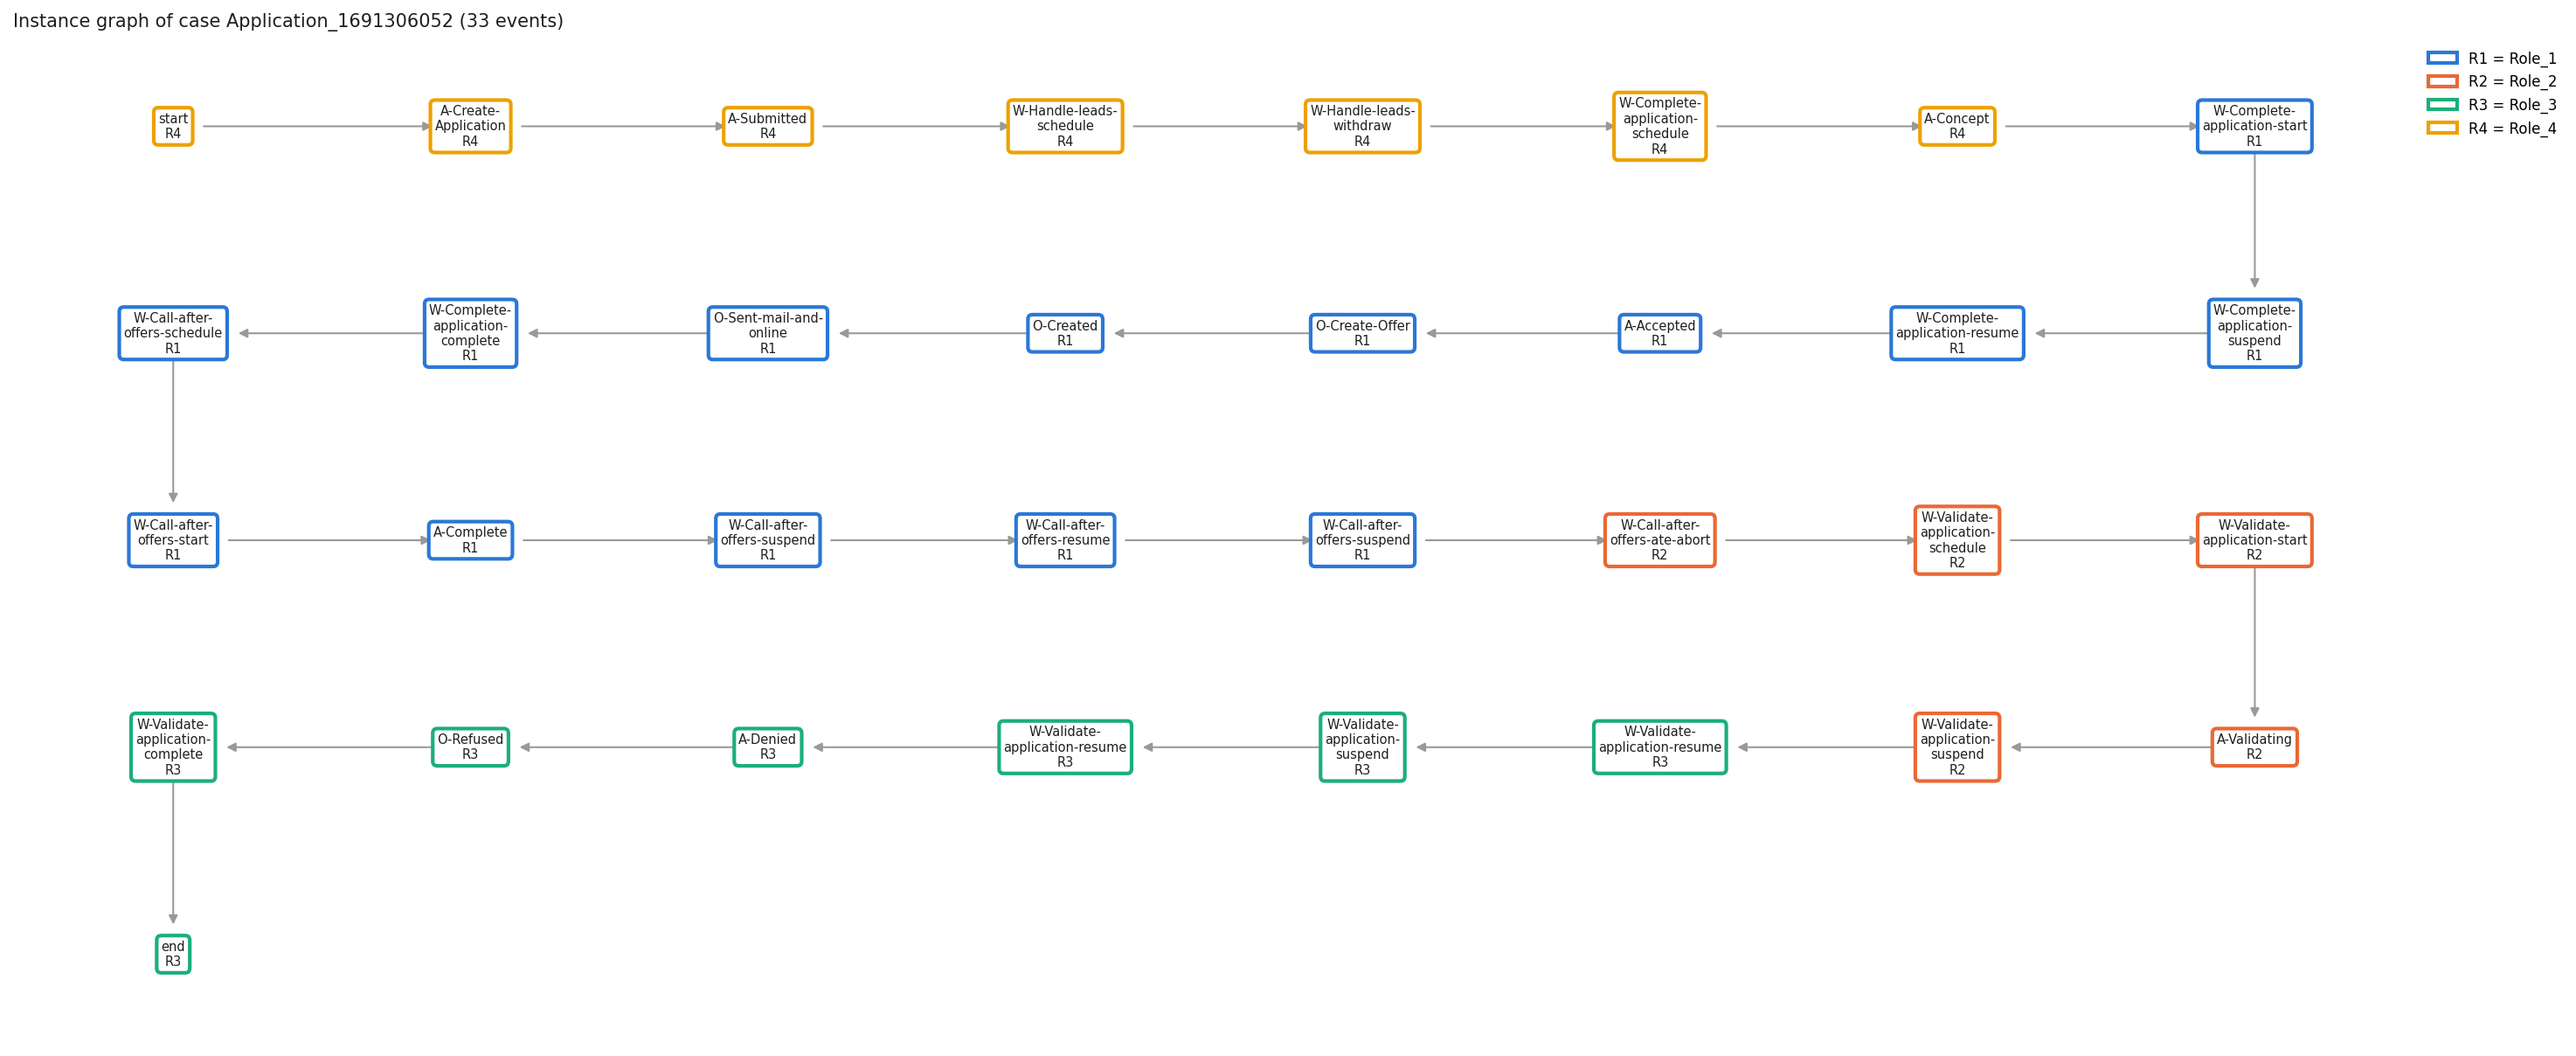
\includegraphics[width=\textwidth]{figures/instance_graph_example.png}
\caption{Instance graph of one case (read as a snake: left to right, then right
to left). Border colour and tag show the role: intake (R4), offer team (R1),
validation (R2) and decision (R3).}
\label{fig:ig}
\end{figure}

\paragraph{Patterns.} SUBDUE starts from 541 one-edge patterns. A single
iteration returns 20 overlapping variants of one sequence (54--80\% of the
cases): the beam search keeps refining the same region of the graph. The
hierarchical run finds a different process phase in every iteration
(Table~\ref{tab:patterns}). Patterns P1.1 and P2.1 (Figure~\ref{fig:patterns})
are handovers: after calling the customer about the offer, the offer team
(Role\_1) hands the case over to the validation team (Role\_2), in 61\% of the
cases; and the intake (Role\_4) hands over to Role\_1 to complete the
application, in 45\%. Over all instance graphs, 80--93\% of the edges stay
within a role (Figure~\ref{fig:handover}); the main handovers are
Role\_4$\to$Role\_1 (16\% of Role\_4's edges), Role\_5$\to$Role\_3 (17\%),
Role\_2$\to$Role\_3 (9\%) and Role\_1$\to$Role\_2 (7\%).

\begin{table}[t]
\centering
\caption{Best pattern of each of the 10 SUBDUE iterations (beam 4).}
\label{tab:patterns}
\small
\begin{tabular}{llrlr}
\toprule
Pattern & What it shows & Edges & Roles & Cases \\
\midrule
P1.1 & Offer team calls after the offer, validation takes over & 10 & R1, R2 & 61\% \\
P2.1 & Intake registers the application, R1 continues & 7 & R1, R4 & 45\% \\
P3.1 & Offer accepted, created and sent & 3 & R1 & 82\% \\
P4.1 & Call for incomplete files, validation takes over & 6 & R1, R2 & 23\% \\
P5.1 & Validation started & 3 & R2 & 33\% \\
P6.1 & Application completed (concept) & 2 & R1 & 40\% \\
P7.1 & Denied, offer refused, case ends & 3 & R3 & 31\% \\
P8.1 & Offer refused, validation aborted & 2 & R3 & 38\% \\
P9.1 & Completion suspended and resumed & 2 & R1 & 29\% \\
P10.1 & Customer called after the offer & 2 & R1 & 37\% \\
\bottomrule
\end{tabular}
\end{table}

\begin{figure}[t]
\centering
\begin{subfigure}{\textwidth}
  \centering
  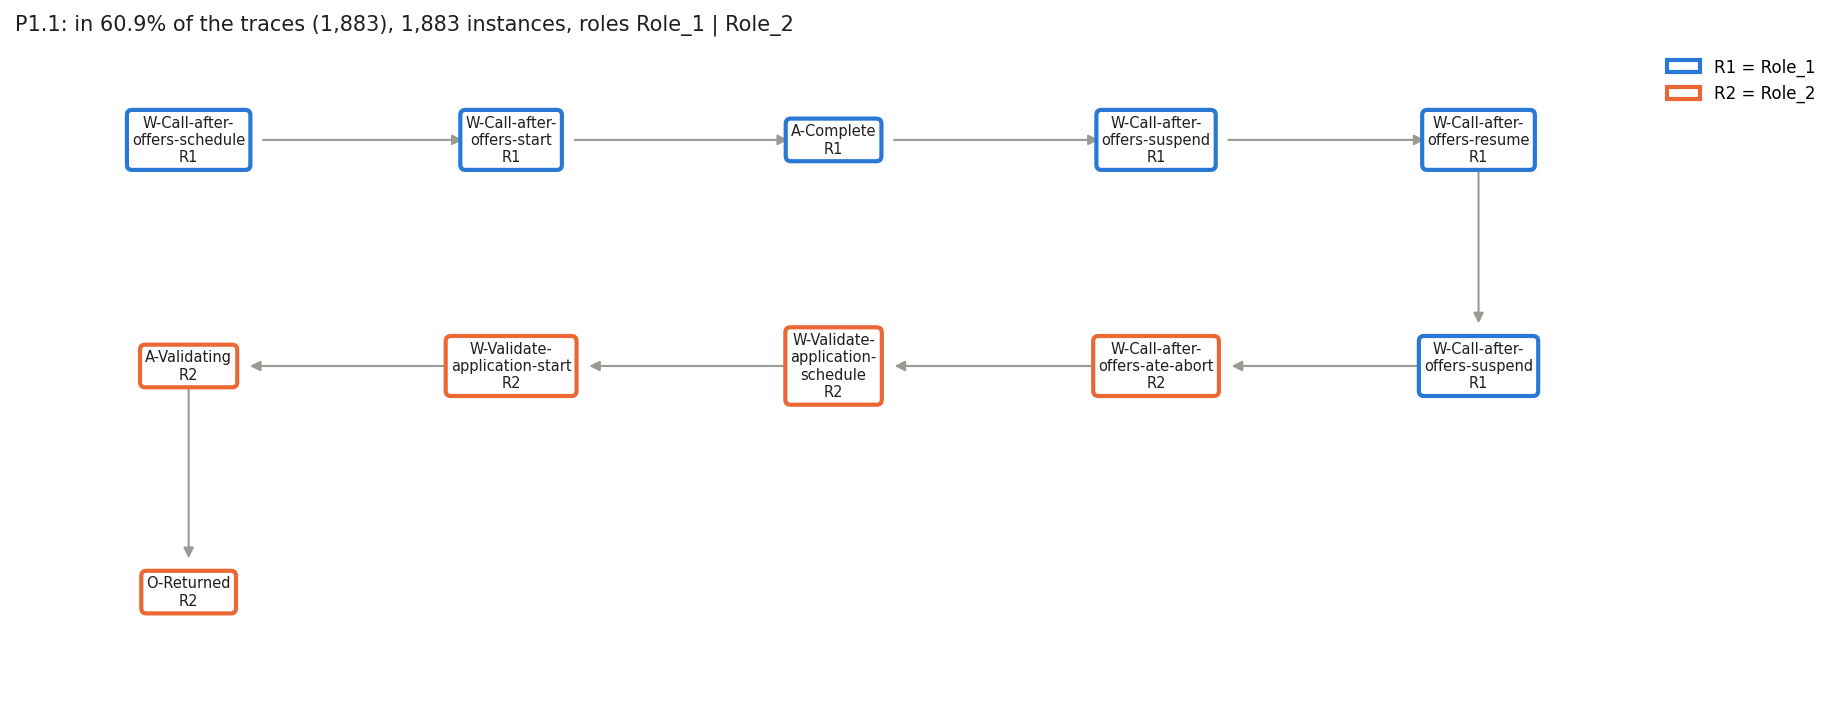
\includegraphics[width=0.9\textwidth]{figures/pattern_P1_1.png}
  \caption{P1.1: handover from the offer team (R1) to the validation team (R2).}
\end{subfigure}

\vspace{0.5em}
\begin{subfigure}{\textwidth}
  \centering
  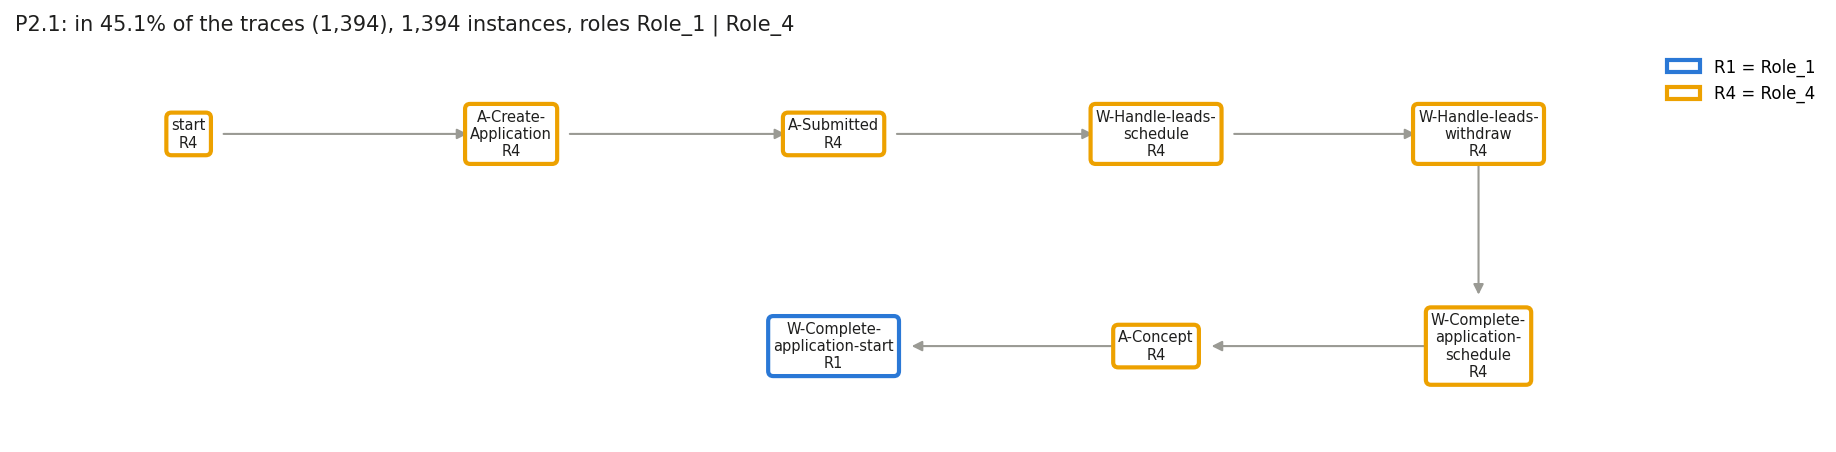
\includegraphics[width=0.9\textwidth]{figures/pattern_P2_1.png}
  \caption{P2.1: handover from the intake (R4) to the offer team (R1).}
\end{subfigure}
\caption{Two discovered behavioral patterns with a handover of work.}
\label{fig:patterns}
\end{figure}

\begin{figure}[t]
\centering
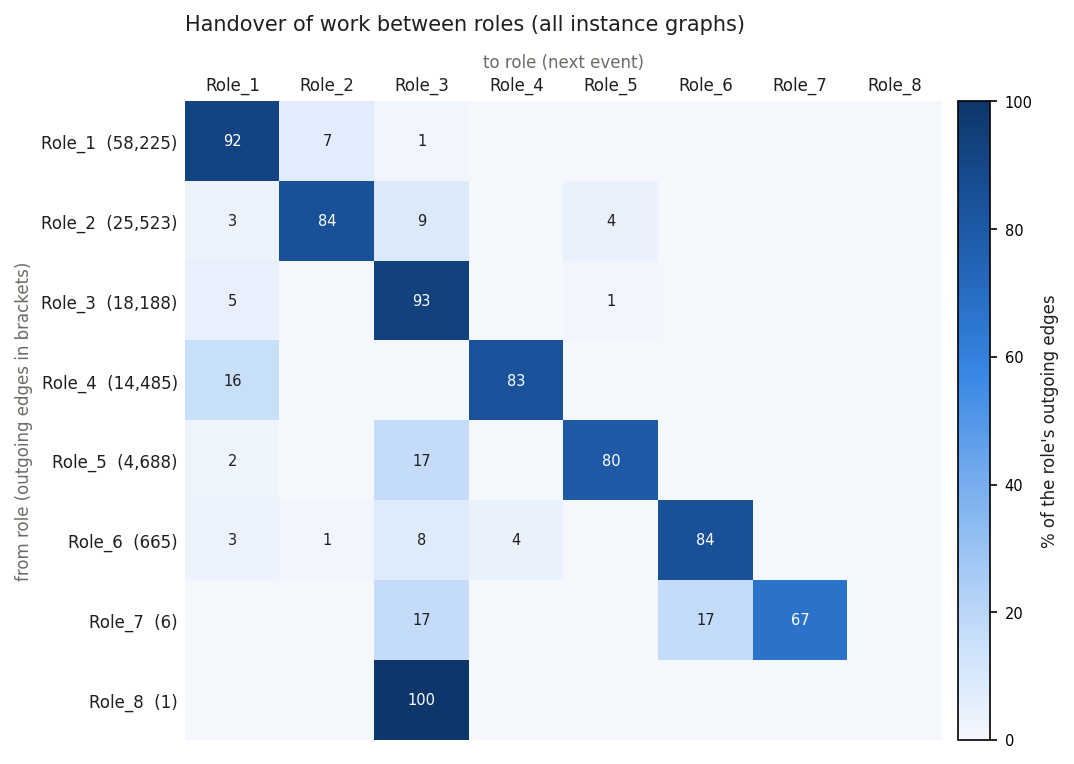
\includegraphics[width=0.62\textwidth]{figures/role_handover.png}
\caption{Handover of work between roles over all instance graphs: share of the
outgoing edges of a role that lead to an event of each role.}
\label{fig:handover}
\end{figure}

\paragraph{Gold standard.} Table~\ref{tab:evaluation} and
Figure~\ref{fig:evaluation} compare the configurations. The single iteration is
precise but finds only 3 of the 9 gold patterns, because its patterns are
variants of one sequence. The hierarchical run finds 8 of 9 (recall 0.89) with
precision 0.63 (F1 0.74). \emph{Failed cases:} G8 (incomplete files) is missed
because its activities are split between Role\_2 and Role\_3 (37\% and 55\%),
which spreads the behaviour over several labels. Of the 11 discovered patterns
counted as incorrect, several are plausible practices that the gold standard
does not contain (e.g.\ P8.1, a denial variant), and P6.1 contains
\texttt{A-Concept} performed by Role\_1, whereas the gold standard assigns this
activity to Role\_4; it is in fact shared 46/53\% between the two roles.
The baseline of frequent paths reaches a similar score (F1 0.72--0.80 for
paths of 3--4 edges). Because the instance graphs are almost purely sequential,
the advantage of graph mining, representing parallel behaviour compactly, cannot
show here.

\begin{table}[t]
\centering
\caption{Discovered patterns against the gold standard (pattern and edge level).
Beam 10 and 20: see the note in the text.}
\label{tab:evaluation}
\small
\begin{tabular}{lrrrrrr}
\toprule
Method & Patterns & Precision & Recall & F1 & Edge prec. & Edge rec. \\
\midrule
SUBDUE, 1 iteration (beam 4) & 20 & 1.00 & 0.33 & 0.50 & 0.46 & 0.29 \\
SUBDUE, 10 iterations (beam 4) & 30 & 0.63 & 0.89 & 0.74 & 0.42 & 0.88 \\
SUBDUE, 10 iterations (beam 10) & 30 & tbd & tbd & tbd & tbd & tbd \\
SUBDUE, 10 iterations (beam 20) & 30 & tbd & tbd & tbd & tbd & tbd \\
Frequent paths, 2 edges & 30 & 0.37 & 0.78 & 0.50 & 0.44 & 0.88 \\
Frequent paths, 3 edges & 30 & 0.60 & 0.89 & 0.72 & 0.43 & 0.88 \\
Frequent paths, 4 edges & 30 & 0.73 & 0.89 & 0.80 & 0.41 & 0.88 \\
\bottomrule
\end{tabular}
\end{table}

\begin{figure}[t]
\centering
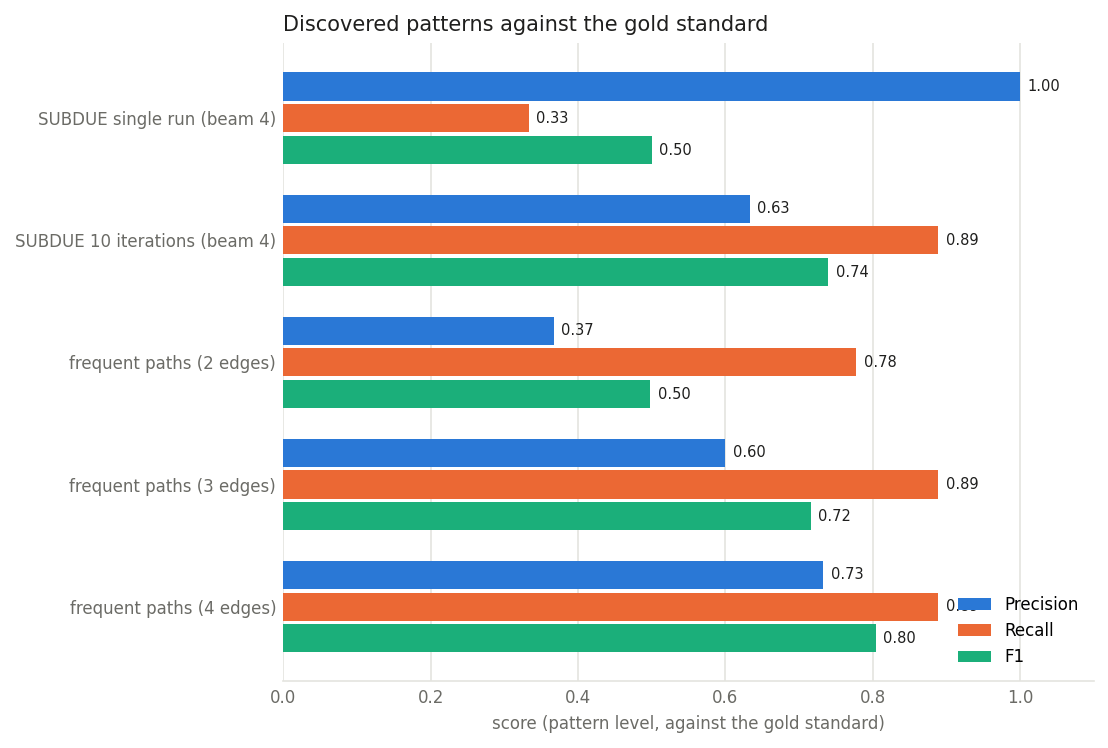
\includegraphics[width=0.75\textwidth]{figures/evaluation.png}
\caption{Precision, recall and F1 of SUBDUE and the frequent-path baseline.}
\label{fig:evaluation}
\end{figure}

% =====================================================================
\section{Limitations and Future Work}\label{sec:limitations_futurework}

\paragraph{Process model.} The Inductive Miner in pm4py~2.2.16 finds almost no
parallelism on this log, even without roles, so the instance graphs are
sequences and the patterns are sequential. This removes the main advantage of
instance graphs over traces~\cite{diamantini2016behavioral}, and explains why a
frequent-path baseline performs as well as SUBDUE. Future work: derive the
causal relations from another miner or from the activity-level model and lift
them to the role labels.

\paragraph{Roles.} The dominant-role assignment creates very small roles (Role\_7
and Role\_8) and one large role (Role\_1, 86 users) that probably merges
several functions. A higher similarity threshold, or assigning roles per event
instead of per resource, should be evaluated. Activities shared by roles (e.g.\
\texttt{A-Concept}, incomplete files) fragment patterns.

\paragraph{Gold standard.} The gold standard is small (9 patterns), written by
ourselves after seeing preliminary results, and partly uses the role table of
our own step~1. Precision is underestimated where plausible patterns are
missing from it. Future work: a synthetic log with injected work practices and
known roles, as in~\cite{diamantini2016behavioral}, which gives an objective
ground truth, and the structural measures of the paper (coverage, diversity).

\paragraph{Search.} SUBDUE's beam search returns overlapping variants within an
iteration, and its value function favours long sequences. More iterations,
or reporting only maximal patterns, make the result more diverse.

\paragraph{Conclusion.} We implemented behavioral pattern mining from instance graphs for
organizational analysis. Grouping resources into discovered roles makes the
approach tractable on a real log and yields interpretable work practices,
including handovers between teams. A hierarchical SUBDUE search finds most
expected work practices, while the discovered process model, rather than the
pattern miner, is the bottleneck for revealing parallel collaboration.

\printbibliography

\section{Technology Statement}
During the preparation of this work, I/We used [NAME TOOL / SERVICE / VERSION OF AI
TOOL] in order to [REASON]. The following parts of the assignment were
affected/generated by AI tool usage: [INTRODUCTION / METHODS / xxx, DISCUSSION].
After using this tool/service, [NAME STUDENT(S)] evaluated the validity of the tool's
outputs, including the sources that generative AI tools have used, and edited the
content as needed. As a consequence, [NAME STUDENT (S)] take(s) full responsibility
for the content of their work

\end{document}
